\fancychapter{\ac{ai} for \emph{Sueca}}
\label{chapter:artificial-player}

This section will describe the most relevant implementation details of the artificial player.
After thoroughly analysing state-of-the-art techniques to solve imperfect information games, and considering \emph{Sueca} is, at this moment, computationally unsolved, the chosen approach was \ac{pimc}.
To implement this search technique, there are three key concepts or algorithms that require a full understanding: the Information Set, the PICM Search and the MinMax Algorithm.
Moreover, the encountered drawbacks are also further described, as well as the enhancements implemented to overcome those limitations.

\section{Implementing \ac{pimc}}
\label{sec:implementing}

After thoroughly analysing state-of-the-art techniques to solve imperfect information games, and considering \emph{Sueca} is, at this moment, computationally unsolved, the chosen approach was \ac{pimc}.
To implement this search technique, there are three key concepts or algorithms that require a full understanding: the Information Set, the \ac{pimc} and the MinMax Algorithm.
Moreover, the encountered drawbacks are also further described, as well as implemented enhancements to overcome those limitations.


\subsection{Information Set}
An information set represents all the visible information during a game, and also inferred information based on certain events.
The player must keep an instance of the information set per game and update it when necessary.
It stores the known hand of the player and a deck with all the cards whose owner is unknown.
As a result, each time another player plays a card, it should be removed from that deck.

The purpose of managing unplayed cards is to sample possible card distributions for the other three players with their real conditions.
These sampled distributions will be used during the \ac{pimc} search and the closer they are to the real world, the better the search returning value will be.
Additionally, the information set keeps track of suits per player and, when a player does not follow the leadsuit of a trick, it removes that suit from the player possible suits.
By possessing this information, sampling possible distributions gets even closer to the real world, however it increases the complexity of the sampling process.
The sampling method builds a \ac{csp} where:
\begin{itemize}
\item variables are the unplayed cards;
\item each domain is the set of players that still have that suit;
\item and the constraints are the number of times a player can be assigned to a card.
\end{itemize}


\subsection{\ac{pimc} Search}
The following pseudo-code of the \ac{pimc} search algorithm guided the implementation.

\begin{algorithm}
	\caption{PIMC search algorithm}
	\begin{algorithmic}[1]
		\Procedure{PIMC}{InfoSet $I$, int $N$}
			\ForAll {$m \in$ Moves($I$)}
				\State $val[m]$ = 0
			\EndFor
			\ForAll {$i \in \{ 1..N\}$}
				\State $x$ = Sample($I$)
				\ForAll {$m \in$ Moves($I$)}
					\State $val[m]$ += PerfInfoValue($x$, $m$)
				\EndFor
			\EndFor
			\State \textbf{return} $\underset{m}{argmax}\{ val[m] \}$
		\EndProcedure
		\label{alg:pimc}
	\end{algorithmic}
\end{algorithm}

To recapitulate the main points of this algorithm, considering it can choose up to \#Moves($I$), it samples $N$ possible card distributions for the other three players and calculates the reward of playing each possible move for the $N$ sampled worlds.
The returned move is the one that gave more accumulated reward.

The number of iterations this algorithm perform is imposed by the $N$ parameter.
Another version of the algorithm, instead of limiting the number of iterations, specifies the execution time of the main loop.


\subsection{MinMax Algorithm}
As mentioned above, \ac{pimc} has to calculate the reward of playing a card, for each sampled world (line 7 of Algorithm~\ref{alg:pimc}).
Since a sampled distribution assigns the remaining cards to players, every game can be handled as a perfect information game.
Therefore, to compute a perfect information game, considering each player or team intends to win, the MinMax algorithm was used.

MinMax is a popular algorithm for calculating optimal decisions in multiplayer games.
Each node corresponds to a possible move by a player and their successors correspond to the possible moves of the next player.
The player representing the agent and his team mate are both \emph{max} players, likewise, the other two opponents are \emph{min} players.

The complete game tree has 40 levels, from $l_{0}$ to $l_{39}$, and each group of $l_{4n}$ to $l_{4n+3}$ represents a trick.
Additionally, since the utility value can only be determined in terminal nodes, these back-propagate their best or worst child utilities, if they are \emph{max} or \emph{min} nodes, respectively.
The utility function to evaluate a sequence of moves deserved a serious consideration and is further detailed in Section~\ref{sec:parametrizing}.


\subsection{Drawbacks and enhancements}
When applying \ac{pimc} to decide which move \emph{m} to make, the number of computed game trees is \#Moves($I$) times $N$ (the number of different distributions), and the size of each game tree depends on the moves that are left to finish the game.
Additionally, the algorithm tends to choose a near optimal decision as long as the $N$ is reasonably large.
As a result, this algorithm has to process a large number of nodes to make a proper decision, specially in the beginning of the game, and, without the enhancements further described, this task was impractical.

\citet*{Russell2009} suggested that MinMax performance can be improved using the alpha-beta prunning, a move ordering heuristic, and a transposition table.
The alpha-beta prunning, by simply storing the best choices so far for the max and min nodes, does not explore nodes that will not influence the final decision.

This technique can also be improved with a favourable ordering heuristic that produces earlier alpha-beta cuts.
Therefore, the implemented ordering heuristic is dynamic and uses an auxiliary computation to decide how to order moves.
Similarly to a human player reasoning, it analyses the current trick and tries to anticipate its winner.
If this auxiliary procedure expects the winner to be one of its opponents, it orders the cards from the less valuable to the most valuable, otherwise, it does the opposite.
This concept might bring a trade-off between the produced speed and the time spent on this extra computation plus the sort.
However, alpha-beta cuts have reasonably increased and reduced significantly the exploration time of the whole tree.
\todo[inline]{Se houver tempo, quantificar a perfomance atingida com esta heuristica. FOI BRUTAL!}

Another improvement with remarkable results on the MinMax performance was a transposition table.
Considering each card configuration or distribution will produce \#Moves($I$) game trees, they will contain sufficient similar subtrees to store their first computed values.
Therefore, instead of recomputing them, they can be reused.
\todo[inline]{Detail time versus space problems. Too many days wasted on that deserves it!}

Furthermore, another heuristic was used, aiming to reduce redundancy in the state generation, suggested by \citet{Buro}.
When computing Moves($I$), two or more cards of the same suit, with consecutive ranks and with the same value can be considered as the same move, since they produce the same value.
For instance, holding 3$\clubsuit$, 4$\clubsuit$ and 5$\clubsuit$ on the same hand will produce three equivalent states and therefore, this heuristic produce only one.

Limiting the maximum depth achieved by the MinMax algorithm was another available option, specially for earlier decisions that produce larger trees and the time to compute them was impractical.
However, considering a non-terminal node as terminal may imply the utility function to be revised or somehow predicted.
Different parametrizations related to the depth cut are detailed further in Section~\ref{sec:parametrizing}

%Lastly, to exploit the computational resources and considering the fact that \ac{pimc} can be easily paralleled, the outer loop was divided into the number of \acp{cpu} the machine has.
%Using a machine with 4 \acp{cpu}, the speed-up is nearly 4.
%The only concern while paralleling this algorithm is to carefully manage the scope of shared and private variables among the threads.












\section{Measuring parametrization effects}
\label{sec:parametrizing}

After implementing the \ac{pimc} search previously described, some tests were executed in order to observe the effects of different parametrizations.
However, these tests had to be comparative and a baseline or benchmark was required to establish a standard measure.


\subsection{Creating benchmarks}
The baseline agent was called Rule-based and its main idea was to chose a move considering predefined rules, instead of using hard computational algorithms.
The following pseudo-code illustrates the deliberation process of this agent and tries to roughly reproduce the reasoning of a non-professional human player.

\begin{algorithm}
	\caption{Rule-based Sueca algorithm}
	\begin{algorithmic}[1]
		\Procedure{RuleBasedDecision}{InfoSet $I$}
			\State $HighestCardPerSuit$ = GetHighestCardPerSuitFromHand($I$)
			\ForAll {$h \in HighestCardPerSuit$}
				\If{isHighestUnplayedFromSuit($h$)}
					\If{GetSuit($h$) = TRUMP \&\& CountCardsFromSuit($I$) > 5}
						\State \textbf{return} h
					\ElsIf{GetSuit($h$) $\not=$ TRUMP \&\& CountCardsFromSuit($I$) > 5}
						\State \textbf{break}
					\ElsIf{GetSuit($h$) $\not=$ TRUMP}
						\State \textbf{return} h
					\EndIf
				\EndIf
			\EndFor
			\State \textbf{return} GetLowestCardFromHand($I$)
		\EndProcedure
	\end{algorithmic}
	\label{alg:pimc}
\end{algorithm}

It starts by collecting the highest cards of each allowed suit for the current play.
The possibility of playing such a highest card is granted by two requirements: being the highest unplayed card of that suit; and not holding at least other 5 cards from that suit, except for the trump suit.
Otherwise, this rule-based player return the lowest possible card.

The first experiments to test this baseline player compare three different scenarios:
\begin{itemize}
\item (a) 1000 games with 4 Rule-based players [dark green];
\item (b) 1000 games with 1 Rule-based player and 3 Random players [red];
\item (c) 1000 games with 2 Rule-based players against 2 Random players [dark blue].
\end{itemize}
Each scenario has a corresponding colour that will be used in every chart for the same scenario.

\begin{figure}[h]
        \centering
        \begin{subfigure}[h]{0.32\textwidth}
                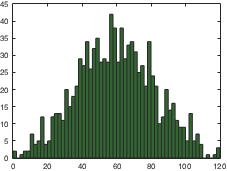
\includegraphics[width=\textwidth]{./img/5/HA-4RuleBased}
                \caption{Scenario A}
                \label{fig:histogramA}
        \end{subfigure}
        \begin{subfigure}[h]{0.32\textwidth}
                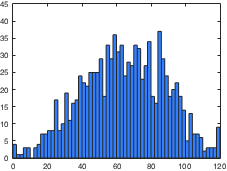
\includegraphics[width=\textwidth]{./img/5/HB-1RuleBased_3Random}
                \caption{Scenario B}
                \label{fig:histogramB}
        \end{subfigure}
        \begin{subfigure}[h]{0.32\textwidth}
                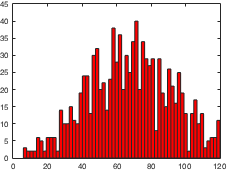
\includegraphics[width=\textwidth]{./img/5/HC-2RuleBased_2Random}
                \caption{Scenario C}
                \label{fig:histogramC}
        \end{subfigure}
        \caption[Histograms of the final points obtained in the 3 scenarios]{Histograms of the final points obtained in 1000 games by: (a) one of the teams; (b) the team with 1 Rule-based player and 1 Random player; (c) the team with 2 Rule-based players}
        \label{fig:histograms}
\end{figure}

The histograms presented on Figure~\ref{fig:histograms} exhibit the distribution of final points in 1000 games by one of the teams in each scenario.
However, comparing the three histograms gets easier when merging the three fitting curves in one graph, Figure~\ref{fig:fitHistABC}.

\begin{figure}[h!]
  \centering
    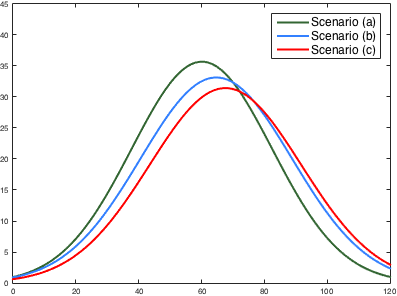
\includegraphics[width=0.5\textwidth]{./img/5/FitHistABC}
  \caption{Fitting curves of histograms presented on Figure~\ref{fig:histograms} with the same colour scheme}
\label{fig:fitHistABC}
\end{figure}

In scenario (a), results were very balanced, as expected, because all players had the same deliberation process.
In 1000 games one of the teams obtained a winning percentage of 48.5\%, a drawing percentage of 1.9\% and a losing percentage of 49.6\%.
The scenario (b) showed that a team with 1 Rule-based player and 1 Random player can beat a 2 Random players team with a winning percentage of 51.6\%, a drawing percentage of 1.8\% and a losing percentage of 41.6\%.
Finally, in scenario (c), the team with 2 Rule-based players beat the the 2 Random players with the highest winning percentage of 61.1\%, a drawing percentage of 1.8\% and losing percentage of 37.1\%.

A player's performance can only be measured when playing with different players, otherwise, playing a considerable amount of games will balance the winning and losing rates, as seen in scenario (a).
Additionally, theses results also demonstrated the impact of the team player on the team score, since having 2 Rule-based players in the same team increased the winning rate of the team with only 1 Rule-based player.

In addition to these conclusions, the winning rates achieved by 1 Rule-based (scenario (b)) and 2 Rule-based (scenario (c)) were lower than expected, since their opponents have completely random procedures for playing the game.
A possible reason might be \emph{Sueca}'s element of chance, which means certain hands can limit the result even though the opponents are Random players.

This idea incited some research on the influence of the players' initial conditions on the game result.
On one hand, the power of a hand is completely dependent on the playing manner of each player, and therefore, using Random players to measure this property is inappropriate.
On the other hand, this measure will not be used to carefully predict a hand's effect on the final result.
Instead, its goal is to generally classify a hand in one out of three distinct categories (\emph{hard}, \emph{medium} and \emph{easy}) and to filter the hands that are hardly or easily capable of winning.
As a result, the chosen scenario to extract these categories' features was (a).

In order to derive such characteristics, the first step is to presume and collect possible features of the initial game conditions that may influence the final result.
After that, computing a linear regression on that data to decide the relevant features.
In the first iterations of this process, many variables were tested for one player of the team and also for both.
For instance, the total points, the trump points, the number of aces, the number of sevens, the number of trumps, being the first to play, having the trump ace, the number of suits.
However, many of them were rejected by the null hypothesis with a significance level of 0.05, and the remaining features were only three: team aces number, team sevens number and team trumps number.

\begin{figure}[h!]
  \centering
    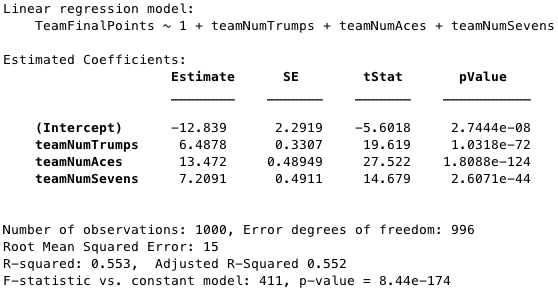
\includegraphics[width=0.7\textwidth]{./img/5/linearRegression}
  \caption{Linear regression with the \emph{team aces number}, the \emph{team sevens number} and the \emph{team trumps number} as predictor variables and \emph{team final points} as the response variable}
\label{fig:linearRegression}
\end{figure}

Figure~\ref{fig:linearRegression} shows the detailed statistic relationship of the mentioned variables on the team final result.
Although the model has a low r-squared value, the p-values of the predictors can reject their null hypothesis and prove their importance in the final result.

\begin{figure}[h]
        \centering
        \begin{subfigure}[h]{0.32\textwidth}
                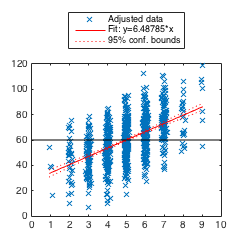
\includegraphics[width=\textwidth]{./img/5/teamTrumpsNumber}
                \caption{Variable \emph{team trumps number}}
                \label{fig:teamTrumpsNumber}
        \end{subfigure}
        \begin{subfigure}[h]{0.32\textwidth}
                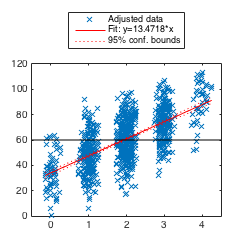
\includegraphics[width=\textwidth]{./img/5/teamAcesNumber}
                \caption{Variable \emph{team aces number}}
                \label{fig:teamAcesNumber}
        \end{subfigure}
        \begin{subfigure}[h]{0.32\textwidth}
                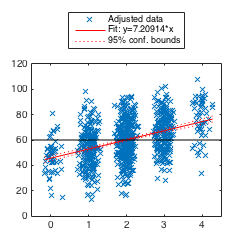
\includegraphics[width=\textwidth]{./img/5/teamSevensNumber}
                \caption{Variable \emph{team sevens number}}
                \label{fig:teamSevensNumber}
        \end{subfigure}
        \caption{Fitting function for each individual predictor variable}
        \label{fig:fitFunctions}
\end{figure}

Finally, Figure~\ref{fig:fitFunctions} can help to quantify the importance of each feature and to build the domain values for each class (\emph{hard}, \emph{medium} and \emph{low}).
Regarding the Figure~\ref{fig:teamTrumpsNumber}, the numbers of initial trumps held by a team, where at least 60\% of the samples were lost games, are 1, 2, 3 and 4..
In the same way, the numbers of initial trumps held by a team, where ate least 60\% of the samples were won games, are 6, 7, 8 and 9.
Applying the same procedure to the three predictor variables, the decided \emph{hard} initial conditions to a team (with low probability of winning) are to have at most 4 trumps, at most 1 ace and at most 1 seven.
Conversely, the decided \emph{easy} initial conditions to a team (with high probability of winning) are to have at least 6 trumps, at least 3 ace and at least 3 seven.
Other cases are considered as \emph{medium} hands.

The developed classifications will be used in two different measures: (1) the \ac{fgr}, which means the percentage of won or drew games; (2) the histogram of obtained points by a certain team.
The first measure is more general and is used to compare the effective performance of players.
On the other hand, the second measure details the points distribution, since the same \acp{fgr} can lead to different histogram of the final points.

\begin{figure}[h]
        \centering
        \begin{subfigure}[h]{0.32\textwidth}
                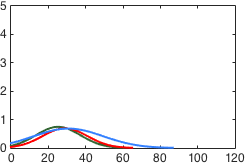
\includegraphics[width=\textwidth]{./img/5/ABChard}
                \caption{filipa}
                \label{fig:ABC-Hhard}
        \end{subfigure}
        \begin{subfigure}[h]{0.32\textwidth}
                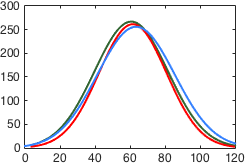
\includegraphics[width=\textwidth]{./img/5/ABCmedium}
                \caption{filipa}
                \label{fig:ABC-Hmedium}
        \end{subfigure}
        \begin{subfigure}[h]{0.32\textwidth}
                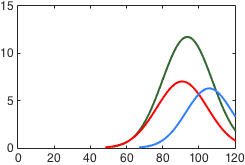
\includegraphics[width=\textwidth]{./img/5/ABCeasy}
                \caption{filipa}
                \label{fig:ABC-Heasy}
        \end{subfigure}
        \caption{filipa}
        \label{fig:ABC-CH}
\end{figure}

Figure~\ref{fig:ABC-CH} shows the distribution of the final points obtained in scenarios (a), (b) and (c) divided into the three mentioned classifications.
The goal of dividing Figure~\ref{fig:fitHistABC} is to see if the detected differences play a prominent role in each individual initial hand type.
However, out of each 1000 collected games, a few percentage refers to games with \emph{hard} or \emph{easy} initial conditions (between 2\% and 3\% each one), which means the apparent results from \emph{hard} and \emph{easy} initial conditions have low confidence values.
The final points of a team are higher as its Gaussian fitting curve moves to the right in the x axe.
Hence, the distribution charts for \emph{hard} and \emph{medium} evidence the same results: the team with 1 Rule-based player (b) achieved higher final scores and the team with 2 Ruled-based players (c) obtained even higher when compared to 4 Random players (a).
Nevertheless, regarding \emph{easy} initial conditions, the team with 1 Rule-based player underperforms slightly the other two scenarios.

\begin{figure}[h!]
  \centering
    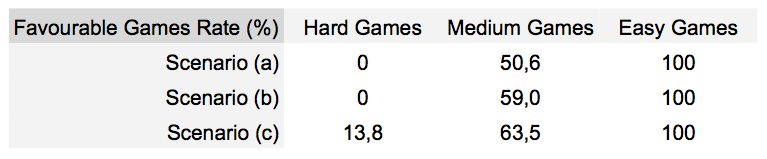
\includegraphics[width=0.7\textwidth]{./img/5/ABC-frg}
  \caption{filipa}
\label{fig:ABC-frg}
\end{figure}

Additionally, the \acp{fgr}, presented in Figure~\ref{fig:ABC-frg}, measure the effectiveness of players when competing with each other.
This rate also evidenced that the Rule-based player outperforms the Random player, mainly based on the \ac{fgr} of the \emph{medium} hands, in which the confidence is higher due to number of samples.

In sum, the Rule-based player guided the development of new measures and will be the benchmark for evaluating the \ac{pimc} algorithm.


\subsection{The Trick Player}

The \ac{pimc} algorithm, implemented as described in Section~\ref{sec:implementing}, cannot explore complete trees until the middle of the game, and therefore, the depth had to be limited.
So, the first two possible parametrizations of the algorithm were the depth limit and the \emph{N} that defines the number of different distributions to be sampled while choosing a card to play.
As a result, two distinct branches were clear, creating a version with a low depth limit and a high \emph{N} value, and another one that has a higher depth limit with lower \emph{N} values.
Additionally, the third possible parametrization is the utility function used by the player.

The Trick player, as the name suggests, evaluates only one trick of every game tree (depth limit of 1) and samples 1000 different distributions (\emph{N} value).
Its utility function is modelled by:
\begin{equation} \label{eq:uf1}
u_1 = \left\{
                \begin{array}{ll}
                  currentTeamPoints, & currentTeamPoints \geq otherTeamPoints\\
                  - otherTeamPoints, & currentTeamPoints < otherTeamPoints
                \end{array}
              \right.
\end{equation}

In order to observe the Trick player performance, it will be considered the following scenarios:
\begin{itemize}
\item (d) 1000 games with 1 Trick player and 3 Rule-based players [yellow];
\item (e) 1000 games with 2 Trick players against 2 Rule-based players [orange].
\end{itemize}

The \ac{fgr} of the team with 1 Trick player and 1 Rule-based (d) was 52.8\% (50.5\% won games and 2.3\% drew games), and at the same time, the \ac{fgr} of the team with 2 Trick players (e) was 55.6\% (53.4\% won games and 2.2\% drew games).
In the same way of the difference between scenarios (b) and (c), having two Trick players on the same team significantly improves the results when compared to only one.
This evidence was expected, since \emph{Sueca} is a team game.

\begin{figure}[h!]
  \centering
    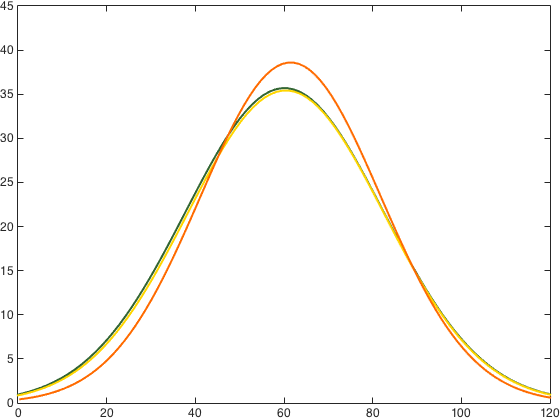
\includegraphics[width=0.5\textwidth]{./img/5/ADE}
  \caption{filipa}
\label{fig:ADE}
\end{figure}

Additionally, Figure~\ref{fig:ADE} presents the distributions of the 1000 obtained final scores from each scenario.
Scenario (a, green) was also included to provide a guide of equilibrium.
The Gaussian fitting curve of scenario (d, yellow) is nearly coincident with the one of scenario (a), suggesting one Trick player in a team does not influence the results.
On the other hand, a team with 2 Trick players, scenario (e, orange), evidences a higher distribution between 60 and 80 points.
These conclusions are also supported by the \acp{fgr} of 50.4\%, 50.5\% and 53.4\% from the teams of scenarios (a), (d) and (e), respectively.

\begin{figure}[h]
        \centering
        \begin{subfigure}[h]{0.32\textwidth}
                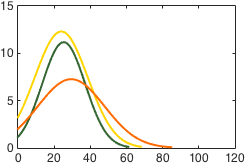
\includegraphics[width=\textwidth]{./img/5/ADEhard}
                \caption{filipa}
                \label{fig:ADEhard}
        \end{subfigure}
        \begin{subfigure}[h]{0.32\textwidth}
                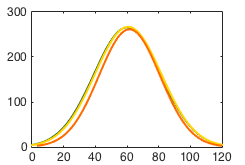
\includegraphics[width=\textwidth]{./img/5/ADEmedium}
                \caption{filipa}
                \label{fig:ADEmedium}
        \end{subfigure}
        \begin{subfigure}[h]{0.32\textwidth}
                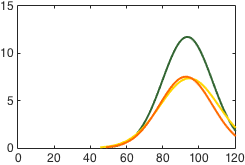
\includegraphics[width=\textwidth]{./img/5/ADEeasy}
                \caption{filipa}
                \label{fig:ADEeasy}
        \end{subfigure}
        \caption{filipa}
        \label{fig:ADE-CH}
\end{figure}

When analysing the Gaussian fitting curves divided into the classes of initial hands, results agree with previous conclusions, except for the \emph{hard} classification of initial conditions.
So, in scenario (e, orange) the team of 2 Trick players achieved higher scores with \emph{hard} and \emph{medium} hands, while with \emph{easy} hands the modal values of the three scenarios seem to be concurrent.
However, as previously mentioned, out of each 1000 collected games, a few percentage refers to games with \emph{hard} or \emph{easy} initial conditions (between 2\% and 3\% each one), which means the apparent results from \emph{hard} and \emph{easy} initial conditions have low confidence values.

\begin{figure}[h!]
  \centering
    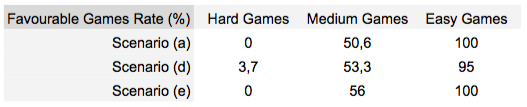
\includegraphics[width=0.7\textwidth]{./img/5/ADE-frg}
  \caption{filipa}
\label{fig:ADE-frg}
\end{figure}

Moreover, the \acp{fgr} in Figure~\ref{fig:ADE-frg} evidenced that the Trick player slightly outperforms the Rule-based player, mainly based on the \ac{fgr} of the \emph{medium} hands, in which the confidence is higher due to number of samples.
The unexpected differences on scenario (d) with both \emph{hard} and \emph{easy} initial conditions refer to only one game, in both cases, and may reflect some flaws on the classification inferred from the linear regression.



















